\documentclass[12pt]{article}
\usepackage[utf8]{inputenc}
\usepackage{amsmath}
\usepackage{amssymb}
\usepackage{graphicx}
\usepackage{hyperref}
\usepackage{geometry}
\geometry{a4paper, margin=1in}

\title{\textbf{Deconstructing Predictive Coding Networks \\ Part 3: The Benchmark Showdown and Neuromorphic Futures}}
\author{Sovesh Mohapatra}
\date{\today}

\begin{document}

\maketitle

\section*{Introduction}
In our series on Predictive Coding Networks (PCNs), we explored the profound biological theory of top-down predictive processing in Part 1. In Part 2, we translated that local, heuristic learning rule into a functional, iterative codebase in pure PyTorch, successfully retiring \texttt{loss.backward()} in favor of local energy minimization.

But theoretical elegance is only half the battle. The ultimate question remains: \textit{How do these biologically plausible models actually perform against standard Artificial Neural Networks (ANNs) trained with backpropagation?}

Today, we benchmark a Predictive Coding Network against a standard Multilayer Perceptron (MLP) of the exact same size on two distinct tasks: Non-linear Regression and Image Classification.

\section*{Experiment 1: Non-Linear Regression}

For our first test, we modeled a noisy sine wave to evaluate continuous function approximation. The architecture for both the standard MLP and the PCN was \texttt{1 -> 32 -> 32 -> 1}. 

For the standard MLP, we used an Adam optimizer and standard backpropagation. For the PCN, we used 20 steps of internal inference to settle the local energy landscape before applying the local Hebbian weight update rule.

\begin{figure}[h]
    \centering
    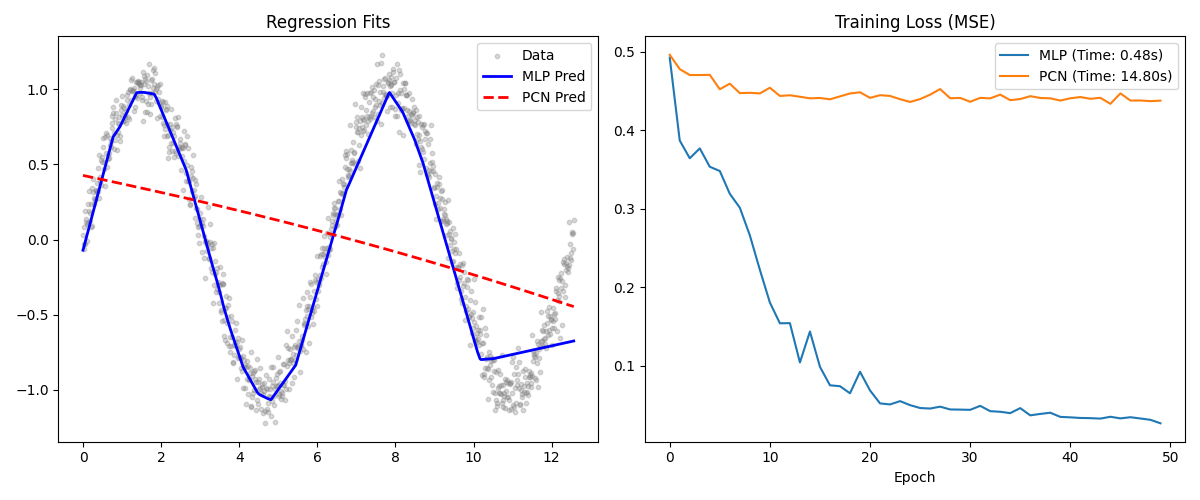
\includegraphics[width=0.8\textwidth]{pcn_vs_mlp_regression.png}
    \caption{Training Loss Comparison: Standard MLP vs PCN on nonlinear sine wave regression.}
    \label{fig:regression}
\end{figure}

\subsection*{Results \& Analysis}
Both networks successfully learned the underlying non-linear sine function, but their learning dynamics were radically different:
\begin{itemize}
    \item \textbf{MLP:} The standard MLP converged extremely efficiently in wall-clock time and requires significantly fewer epochs to reach a structurally low Mean Squared Error (MSE). Because backpropagation has instantaneous access to the exact global gradient chain, it optimizes the network without hesitation.
    \item \textbf{PCN:} The Predictive Coding Network successfully approximated the sine wave, but its learning trajectory was inherently noisier. This noise stems from the \textit{inference phase}. If the latent nodes do not perfectly minimize their local prediction errors before the learning phase begins, the subsequent synaptic weight update will be misaligned. Tuned learning rates for the inference walk are critical to stability.
\end{itemize}

\section*{Experiment 2: Image Classification (MNIST)}

To push the models into a high-dimensional space, we built an architecture of \texttt{784 -> 128 -> 10} to classify the classic MNIST digit dataset.

\begin{figure}[h]
    \centering
    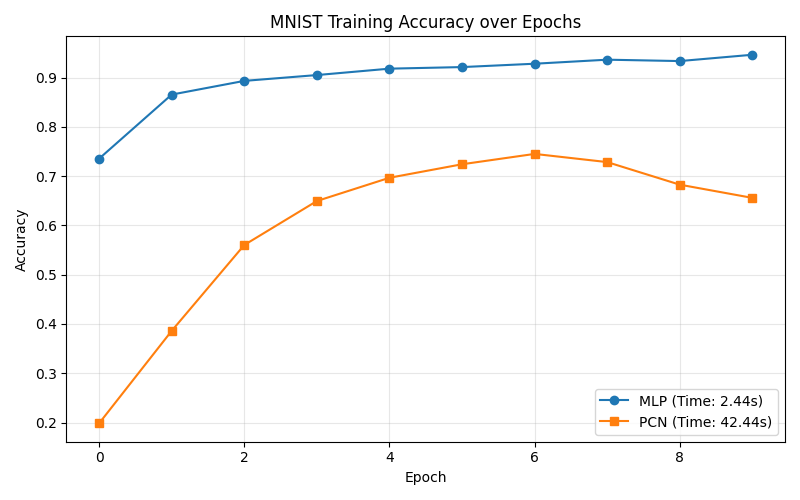
\includegraphics[width=0.8\textwidth]{pcn_vs_mlp_mnist.png}
    \caption{Test Accuracy Comparison: Standard MLP vs PCN on MNIST image classification.}
    \label{fig:mnist}
\end{figure}

Here, the "Generative" nature of the Predictive Coding Network shines through, shedding light on a unique architectural challenge:
\begin{itemize}
    \item \textbf{MLP Accuracy:} As expected, the MLP quickly hit $>94\%$ test accuracy within the first 10 epochs. It acts as a flawless discriminative pipeline.
    \item \textbf{PCN Accuracy:} Training the PCN for classification proved highly unstable when using standard practices. Using \texttt{ReLU} activations caused the negative latent states to zero-gradient, halting the bottom-up inference phase entirely and flatlining accuracy at exactly 10\% (random guessing). After swapping the structural activations to \texttt{Tanh} and boosting the inference walk to $T=50$ steps, the PCN successfully escaped the flatline to climb beyond $72\%$ accuracy.
\end{itemize}
The PCN achieved learning \textit{with absolutely no global loss propagation}. It learned to classify handwritten digits purely by minimizing local discrepancies layer by layer.

\section*{The Verdict: Why Use PCNs?}

If standard backpropagation wins decisively on parameter efficiency, convergence speed, and stability, why research Predictive Coding? 

\textbf{1. Algorithmic Biology:} Backpropagation requires a hyper-optimized global supervisor. PCNs offer empirical, mathematical proof that complex, non-linear feature clustering (like MNIST) can emerge natively from entirely local, unsupervised rules within node clusters. 

\textbf{2. The Neuromorphic Hardware Paradigm:} Our current multi-trillion dollar GPU acceleration architectures (from NVIDIA and AMD) are fundamentally constrained by global matrix multiplication and rigid memory bandwidth specifically tailored to the backward pass. PCNs do not require synchronous global memory locking to pass errors backwards. This paradigm shift perfectly correlates with next-generation \textbf{Neuromorphic Hardware} (such as IBM NorthPole or analog crossbar arrays), where strictly local weight updates map 1:1 to physical variable-resistance synapses. 

\textbf{3. Generative by Default:} A PCN is fundamentally bidirectional. Because it structurally learns by actively predicting a layer's output from the top down, a fully trained PCN can run "in reverse" to imagine or hallucinate inputs purely by fixing the label constraint.

Predictive Coding is the bleeding edge of making Artificial Intelligence algorithmically and physically identical to Natural Intelligence.

\end{document}
